\documentclass[12pt,aspectratio=43]{beamer}

% 自訂字體的封包
\usepackage{fontspec}

% 導入圖形與表格的封包
\usepackage{graphicx}
\graphicspath{{./20251119_Meeting}}

\usepackage{booktabs}

% 排列多個子圖形的封包
\usepackage{subfigure} 

 % 提供進階數學環境與公式排版
\usepackage{mathtools, amsmath, amsfonts, amsthm, latexsym} 

%% 設定中文字體
\usepackage{xeCJK}
\setCJKmainfont[AutoFakeBold=3.5 , AutoFakeSlant=0.2]{標楷體}
\setmainfont{Times New Roman}
\XeTeXlinebreaklocale "zh"
\XeTeXlinebreakskip = 0pt plus 1pt

% 自訂字體顏色的封包
\usepackage{color} 

% 圖表自動編號的封包
\usepackage{caption} 

% 允許表格的一格能多列呈現的封包
\usepackage{multirow} 

% 可指定表格排版的封包
\usepackage{array}

% 翻轉表格的封包
\usepackage{lscape} 

% 序列標號
\usepackage{enumerate} 

%% 設定自動編號
\setbeamertemplate{caption}[numbered]

%% 自訂顏色
\definecolor{Myblue}{RGB}{57,108,144}
\definecolor{Default_Blue}{RGB}{52,51,171}

% (動畫)字會若隱若現的顯示
\beamersetuncovermixins{\opaqueness<1->{45}}{\opaqueness<1->{95}} 

% 設定中文的標籤
\renewcommand{\figurename}{圖} 
\renewcommand{\tablename}{表} 

% 排版形式 
\mode<presentation>{
\usetheme{Berlin}
% enumerate 及 item 的形狀
\setbeamertemplate{itemize items}[triangle]
% 調整外框形式的字體大小
\setbeamerfont{headline}{size=\scriptsize}
\setbeamerfont{footline}{size=\scriptsize}
% 取消右下方的跳轉工具列
\setbeamertemplate{navigation symbols}{} 
% 自定義2：清除外框下緣但僅出頁碼
\setbeamertemplate{footline}[page number] 
% 顏色主題
\usecolortheme{dove}
% 設定頁面邊界
\setbeamersize{text margin left=0.6cm, text margin right=0.6cm}
\special{papersize=\the\paperwidth,\the\paperheight}
\providecommand{\tabularnewline}{\\}
}

\title{Meeting 1119}
\author{黃丞暘}
\institute{國立東華大學應數統計所}
\date{November 19, 2025}

\begin{document}

% 封面
\begin{frame}
  \titlepage
\end{frame}

% 目錄
\begin{frame}{\textbf{Index}}
  \tableofcontents
\end{frame}

% 研究動機 
\section{Research motivation}

\begin{frame}{\textbf{Research motivation}}
\linespread{1.5}
  Semiconductor Manufacturing Process
  \begin{itemize}
    \item Unbox $y = \hat{f}(x)$
  \end{itemize}
  \begin{itemize}
    \item Solution to imbalanced data (differ from SMOTE)
  \end{itemize}
  \begin{itemize}
    \item Fitting model
  \end{itemize}
\end{frame}

% 研究方法
\section{Research method}
\begin{frame}{\textbf{Research method}}
\linespread{1.5}
  \begin{itemize}[]
    \item Features selection
      \begin{enumerate}[]
        \item PCA
        \item NR(p-value)
        \item RF(importance)
      \end{enumerate}
    \item Clustering
      \begin{enumerate}[]
        \item KMeans
        \item AgglomerativeClustering(Hierarchical clustering)
      \end{enumerate}
    \item Model training(StandardScaler, SMOTE)
      \begin{enumerate}
        \item LR, SVM, DT, RF, XGB
        \item ACC, FAR
      \end{enumerate}
  \end{itemize}
\end{frame}

% 結果
\section{Results}

\begin{frame}{\textbf{Results I}　{PCA + KMeans, 2 clusters}}
\linespread{0.9}

\small{$$
\begin{array}{c|cc}
\text{cluster} & 0 & 1 \\
\hline
y=0 & 1460 & 3 \\
y=1 & 103  & 1 \\
\end{array}
$$}

    \begin{center}
        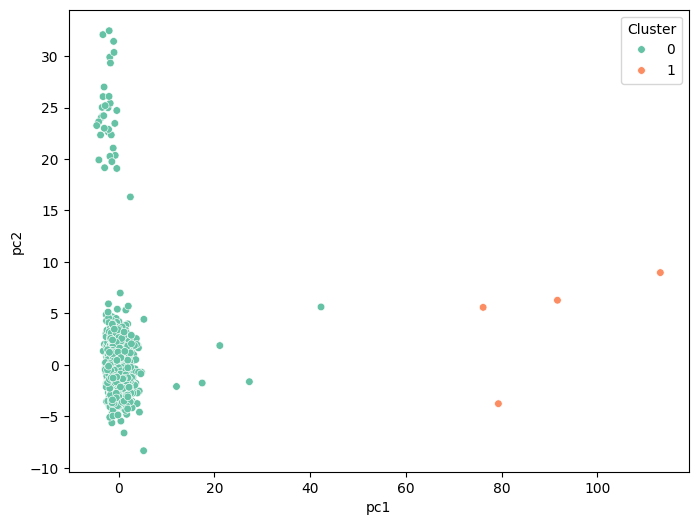
\includegraphics[scale=0.4]{PCA+KMEANS1.png}
    \end{center}

\end{frame}

\begin{frame}{\textbf{Results I}　{Training in cluster 0}}
\linespread{0.9}
{\small
\begin{figure}[h]
\centering

%---------------------- 第一列 ----------------------
\begin{minipage}{0.28\linewidth}
\raggedright
{\small LR}
$$
\small
\begin{bmatrix}
265 & 27 \\
15  & 6
\end{bmatrix}
$$
\end{minipage}
\begin{minipage}{0.28\linewidth}
\raggedright
{\small SVM}
$$
\small
\begin{bmatrix}
292 & 0 \\
21  & 0
\end{bmatrix}
$$
\end{minipage}
\begin{minipage}{0.28\linewidth}
\raggedright
{\small DT}
$$
\small
\begin{bmatrix}
259 & 33 \\
13  & 8
\end{bmatrix}
$$
\end{minipage}

\vspace{0.5em}

%---------------------- 第二列 ----------------------
\begin{minipage}{0.28\linewidth}
\raggedright
{\small RF}
$$
\small
\begin{bmatrix}
292 & 0 \\
20  & 1
\end{bmatrix}
$$
\end{minipage}
\begin{minipage}{0.28\linewidth}
\raggedright
{\small XGB}
$$
\small
\begin{bmatrix}
291 & 1 \\
19  & 2
\end{bmatrix}
$$
\end{minipage}

\end{figure}
}

%---------------------- 第三列：Summary ----------------------
{\small
Summary
$$
\begin{array}{l|cc}
\text{model} & \text{ACC} & \text{FAR} \\
\hline
\text{LR} & 0.8658 & 0.0925 \\
\text{SVM}           & 0.9329 & 0.0000 \\
\text{DT}       & 0.8530 & 0.1130 \\
\text{RF}       & 0.9361 & 0.0000 \\
\text{XGB}            & 0.9361 & 0.0034 \\
\end{array}
$$
}

\end{frame}


\begin{frame}{\textbf{Results II}　{PCA + KMeans, 6 clusters}}
\linespread{0.9}

\small{$$
\begin{array}{c|cccccc}
\text{cluster} & 0 & 1 & 2 & 3  & 4 & 5 \\
\hline
y=0 & 25 & 563 & 627 & 3 & 1 & 244 \\
y=1 & 7 & 36 & 52 & 1 & 0 & 8 \\
\end{array}
$$}

    \begin{center}
        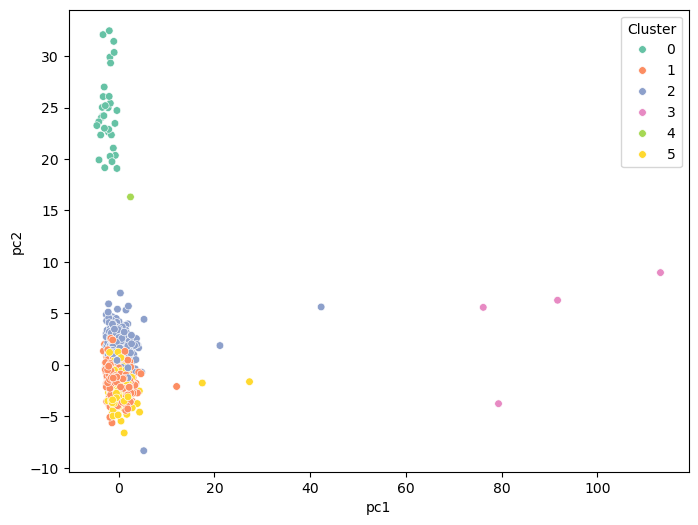
\includegraphics[scale=0.4]{PCA+KMEANS2.png}
    \end{center}

\end{frame}

\begin{frame}{\textbf{Results II}　{Training in cluster 2}}
\linespread{0.9}
{\small
\begin{figure}[h]
\centering

%---------------------- 第一列 ----------------------
\begin{minipage}{0.28\linewidth}
\raggedright
{\small LR}
$$
\small
\begin{bmatrix}
110 & 16 \\
7  & 3
\end{bmatrix}
$$
\end{minipage}
\begin{minipage}{0.28\linewidth}
\raggedright
{\small SVM}
$$
\small
\begin{bmatrix}
126 & 0 \\
10  & 0
\end{bmatrix}
$$
\end{minipage}
\begin{minipage}{0.28\linewidth}
\raggedright
{\small DT}
$$
\small
\begin{bmatrix}
106 & 20 \\
5  & 5
\end{bmatrix}
$$
\end{minipage}

\vspace{0.5em}

%---------------------- 第二列 ----------------------
\begin{minipage}{0.28\linewidth}
\raggedright
{\small RF}
$$
\small
\begin{bmatrix}
126 & 0 \\
9  & 1
\end{bmatrix}
$$
\end{minipage}
\begin{minipage}{0.28\linewidth}
\raggedright
{\small XGB}
$$
\small
\begin{bmatrix}
122 & 4 \\
8  & 2
\end{bmatrix}
$$
\end{minipage}

\end{figure}
}

%---------------------- 第三列：Summary ----------------------
{\small
Summary
$$
\begin{array}{l|cc}
\text{model} & \text{ACC} & \text{FAR} \\
\hline
\text{LR} & 0.8309 & 0.1270 \\
\text{SVM}           & 0.9265 & 0.0000 \\
\text{DT}       & 0.8162 & 0.1587 \\
\text{RF}       & 0.9338 & 0.0000 \\
\text{XGB}            & 0.9118 & 0.0317 \\
\end{array}
$$
}

\end{frame}


\begin{frame}{\textbf{Results III}　{Standard + KMeans, 4 clusters}}
\linespread{0.9}

\small{$$
\begin{array}{c|cccc}
\text{cluster} & 0 & 1 & 2 & 3  \\
\hline
y=0 & 25 & 667 & 3 & 768 \\
y=1 & 7 & 55 & 1 & 41  \\
\end{array}
$$}

    \begin{center}
        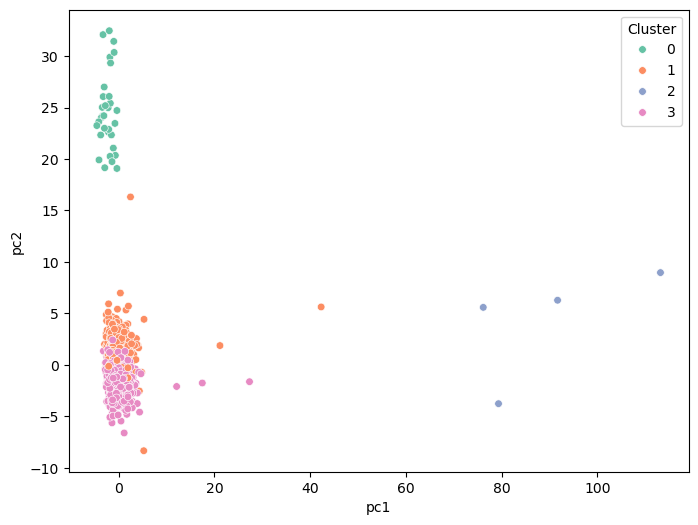
\includegraphics[scale=0.4]{PCA+KMEANS3.png}
    \end{center}

\end{frame}

\begin{frame}{\textbf{Results III}　{Training in cluster 1}}
\linespread{0.9}
{\small
\begin{figure}[h]
\centering

%---------------------- 第一列 ----------------------
\begin{minipage}{0.28\linewidth}
\raggedright
{\small LR}
$$
\small
\begin{bmatrix}
117 & 17 \\
9  & 2
\end{bmatrix}
$$
\end{minipage}
\begin{minipage}{0.28\linewidth}
\raggedright
{\small SVM}
$$
\small
\begin{bmatrix}
134 & 0 \\
11  & 0
\end{bmatrix}
$$
\end{minipage}
\begin{minipage}{0.28\linewidth}
\raggedright
{\small DT}
$$
\small
\begin{bmatrix}
116 & 18 \\
8  & 3
\end{bmatrix}
$$
\end{minipage}

\vspace{0.5em}

%---------------------- 第二列 ----------------------
\begin{minipage}{0.28\linewidth}
\raggedright
{\small RF}
$$
\small
\begin{bmatrix}
134 & 0 \\
11  & 0
\end{bmatrix}
$$
\end{minipage}
\begin{minipage}{0.28\linewidth}
\raggedright
{\small XGB}
$$
\small
\begin{bmatrix}
130 & 4 \\
10  & 1
\end{bmatrix}
$$
\end{minipage}

\end{figure}
}

%---------------------- 第三列：Summary ----------------------
{\small
Summary
$$
\begin{array}{l|cc}
\text{model} & \text{ACC} & \text{FAR} \\
\hline
\text{LR} & 0.8207 & 0.1269 \\
\text{SVM}           & 0.9241 & 0.0000 \\
\text{DT}       & 0.8207 & 0.1343 \\
\text{RF}       & 0.9241 & 0.0000 \\
\text{XGB}            & 0.9034 & 0.0299 \\
\end{array}
$$
}

\end{frame}

\begin{frame}{\textbf{Results IV}　{PCA + AgglomerativeC, 4 clusters}}
\linespread{0.9}

\small{$$
\begin{array}{c|cccc}
\text{cluster} & 0 & 1 & 2 & 3  \\
\hline
y=0 & 1435 & 3 & 24 & 1 \\
y=1 & 96 & 1 & 7 & 0  \\
\end{array}
$$}

\begin{center}
\begin{minipage}{0.45\linewidth}
\centering
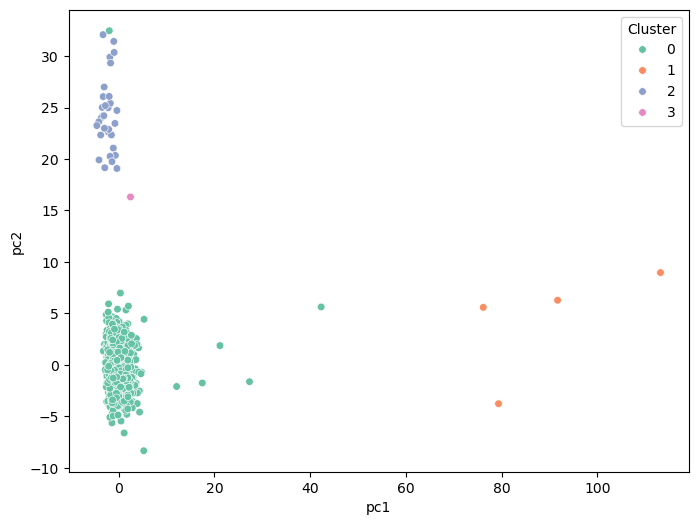
\includegraphics[width=\linewidth]{PCA+KMEANS4.png}
\end{minipage}
\hspace{0.1em}
\begin{minipage}{0.52\linewidth}
\centering
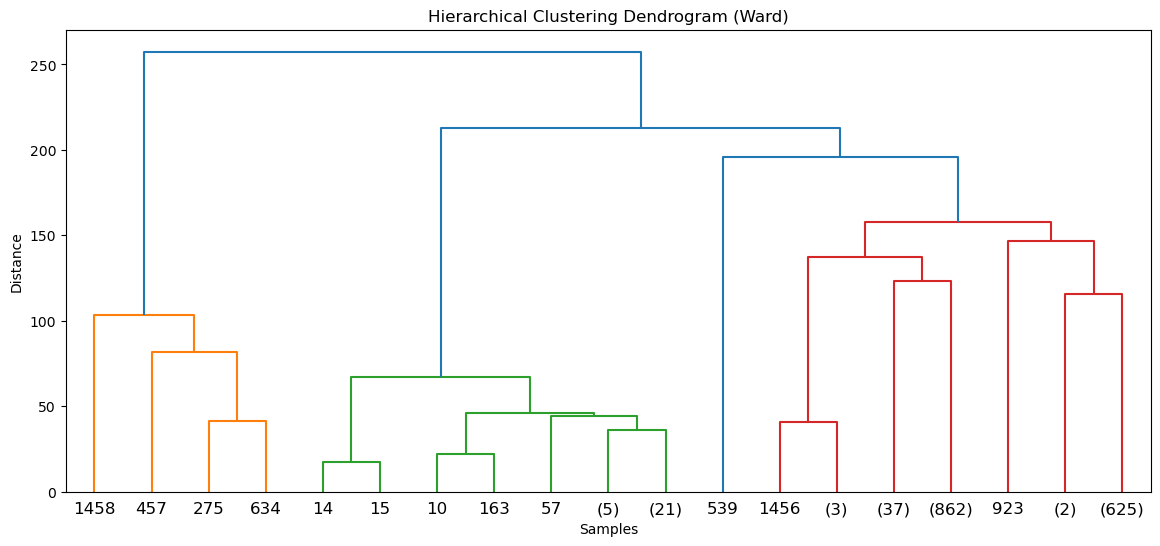
\includegraphics[width=\linewidth]{tree.png}
\end{minipage}
\end{center}

\end{frame}

\begin{frame}{\textbf{Results IV}　{Training in cluster 0}}
\linespread{0.9}
{\small
\begin{figure}[h]
\centering

%---------------------- 第一列 ----------------------
\begin{minipage}{0.28\linewidth}
\raggedright
{\small LR}
$$
\small
\begin{bmatrix}
256 & 32 \\
14  & 5
\end{bmatrix}
$$
\end{minipage}
\begin{minipage}{0.28\linewidth}
\raggedright
{\small SVM}
$$
\small
\begin{bmatrix}
288 & 0 \\
19  & 0
\end{bmatrix}
$$
\end{minipage}
\begin{minipage}{0.28\linewidth}
\raggedright
{\small DT}
$$
\small
\begin{bmatrix}
266 & 22 \\
18  & 1
\end{bmatrix}
$$
\end{minipage}

\vspace{0.5em}

%---------------------- 第二列 ----------------------
\begin{minipage}{0.28\linewidth}
\raggedright
{\small RF}
$$
\small
\begin{bmatrix}
288 & 0 \\
19  & 0
\end{bmatrix}
$$
\end{minipage}
\begin{minipage}{0.28\linewidth}
\raggedright
{\small XGB}
$$
\small
\begin{bmatrix}
288 & 0 \\
19  & 0
\end{bmatrix}
$$
\end{minipage}

\end{figure}
}

%---------------------- 第三列：Summary ----------------------
{\small
Summary
$$
\begin{array}{l|cc}
\text{model} & \text{ACC} & \text{FAR} \\
\hline
\text{LR} & 0.8502 & 0.1111 \\
\text{SVM}           & 0.9381 & 0.0000 \\
\text{DT}       & 0.8697 & 0.0764 \\
\text{RF}       & 0.9381 & 0.0000 \\
\text{XGB}            & 0.9381 & 0.0000 \\
\end{array}
$$
}

\end{frame}

% 參考資料
\section{References}

\begin{frame}{\textbf{References}}
\linespread{1.5}

\footnotesize

\begin{thebibliography}{99}

  \bibitem[Eroglu \& Guleryuz(2025)]{Eroglu2025}
  Eroglu, Y., \& Guleryuz, E. (2025).
  \newblock Enhanced Three-Stage Cluster-Then-Classify Method (ETSCCM).

  \bibitem[Pleli et al.(2024)]{Pleli2024}
  Pleli, A., Baeuerle, S., et al. (2024).
  \newblock Iterative Cluster Harvesting for Wafer Map Defect Patterns.

\end{thebibliography}

\end{frame}

% --- 結束 ---
\section*{結束}

\begin{frame}[plain] % 產生無外框的頁面
	\begin{center}
		{\Huge The End}
		\bigskip\bigskip 

		{\LARGE Questions  \&  Comments}
	\end{center}
\end{frame}
\end{document}ㄒ
